\documentclass[11pt, oneside]{article}   	% use "amsart" instead of "article" for AMSLaTeX format
\usepackage{geometry}
\usepackage{amsmath}              		% See geometry.pdf to learn the layout options. There are lots.
\geometry{letterpaper}                   		% ... or a4paper or a5paper or ...
%\geometry{landscape}                		% Activate for for rotated page geometry
%\usepackage[parfill]{parskip}    		% Activate to begin paragraphs with an empty line rather than an indent
\usepackage{graphicx}				% Use pdf, png, jpg, or eps§ with pdflatex; use eps in DVI mode
								% TeX will automatically convert eps --> pdf in pdflatex
\usepackage{amssymb}

\title{CS 6320 - Project Proposal}
\author{Ally Warner \& Ryan Viertel}
%\date{}							% Activate to display a given date or no date

\begin{document}
\maketitle

\section{Introduction}
A graph is data that is represented with nodes and edges. The nodes are the points of interest and the edges connect and represent the relationship between the nodes. To partition a graph is to divide the graph into smaller components. A good partition is when the number of edges running between separated components is small. In this project, we attempted to partition an undirected sparse graph using the Lanzcos algorithm [3] to find the second small eigenvalues and corresponding eigenvectors.  The principal dataset is available from the University of Florida Sparse Matrix Collection [1]. We tested full reorthogonalization and no orthogonalization as well as different amounts of Lanzcos iterations before partitioning. We visualized the results using Graphviz visualization software [3].

\section{Description of Algorithm}
The principle idea behind our approach to graph partitioning is recursive bisection. We bisect the graph and then recursively bisect each subgraph until there is one subgraph per compute node of the compute cluster partition on which we run our code. Here is an outline of the algorithm.

\begin{enumerate}
	\item Read the matrix from a file in the Matrix Market format and store in memory. This format stores one line for each pair of nodes between which an edge exists. If the matrix is symmetric (as in our case) then it only stores the lower diagonal.

	\item Perform a fixed number of Lanczos iterations to compute the second smallest eigenvalue and corresponding eigenvector of the Laplacian matrix corresponding with our graph. The main step of the Lanczos algorithm, the matrix-vector product, is computed by a ``Black Box'' funtion that accepts as input the adjacency matrix of the graph to be partitioned, and the vector to be used in the product. The matrix-vector product of the laplacian matrix and the vector is then computed in parallel.

	\item The Lanczos iterations produce a tridiagonal matrix whose eigenvalues are approximations of the eigenvalues of the laplacian matrix.  We use the Lapack dsteqr function to compute the eigenvalues and eigenvectors of this matrix, and then compute the Ritz vector corresponding to the second smallest eigenvalue.

	\item The next step is to partition the graph. As per the discussion in class, the eigenvector corresponding to the second smallest eigenvalue of the Laplacian matrix can be used to partition the graph in such a way as to minimize the number of edges crossing the partition.

	\item Finally, we recurse and repeat steps 2-5 on each subgraph. Recursion stops once each compute node has a subgraph and no other compute node is assigned the same subgraph.

	\item Each compute node prints its nodes and edges to a dot file for visualization using graphviz.
\end{enumerate}

\subsection{Parallelization}
There are two main ways in which we have parallelized this application. The first is by parallelizing the Matrix-Vector product. We did this from a shared memory perspective using OpenMP. The second way was by parallelizing the recursion step. We did this from a distributed memory perspective using MPI, each compute node being assigned to one of the two subgraphs generated at each step.

Parallelization of the matrix vector product is straighforward in principle. Each entry of the resulting vector can be computed independently from the others and this can be easly implemented as a CREW procedure. In practice this was a little more difficult due to the minimal storage format of the input matrix. To be able to do the computation in parallel it was necessary to count the number of non-zero entries per row \emph{a priori} and then do a prefix sum on this vector to be able to assign independent chuncks of work to each processor. In the end this step required O(n) work and storage, which is optimal. In addition to parallelizing the Matrix-Vector product, we also parallelized any other independent computations that we could identify.

The distributed memory parallelization that we implemented is admittedly simple and inefficient. Essentially each compute node calculates the Ritz vector individually in each iteration, and then determines which graph nodes to keep for the next iteration. This results in $\log(p)$ steps to partition the graph where p is the number of compute nodes.

\subsection{Possible improvements}
There are several possible improvements to make to the algorithm. In particular, we note the following:

\begin{enumerate}
	\item The biggest improvement that could be made is that rather than having each compute node calculate the Ritz vector individually, the work and memory storage could be split up among nodes to do this in parallel.  Note that for simplicity we elected to parallelize the calculation of the Ritz vectors only from a shared memory perspective.

	\item The second biggest improvement to make would be to use selective reorthogonalization for the Lanczos iteration rather than full reorthogonalization. Since we only needed the second smallest Ritz value, the algorithm converges quickly and full reorthogonalization isn't terribly extensive. This could be improved by reorthogonalizing only when necessary.

	\item There were a couple of minor areas where more parallelization could have been extracted, such as the loop to assign graph nodes to each compute node after the Ritz vector is calculated. These improvements however would have very little effect on the overall performance so for lack of time we decided not to implement them.
\end{enumerate}

\section{Testing \& Analysis}

Timing for the algorithm was tested on 4, 8 and 12 MPI nodes with 10, 20, 40, 80, and 100 Lanzcos iterations with full orthogonalization and no orthogonalization on the matrix shown in Figure 1. The results for the testing is shown in Table 1. During our testing, we have discovered that there is an unknown bug when writing the dot file for visualization in Graphviz [3] in parallel. This yielded unexpected visual results as shown in Figure 2. With this mystery bug, we wanted to at least show proof of concept. Figures 3, 4 and 5 show a small pentagon undirected graph that was partitioned with 2, 3 and 12 processors, respectively, with 100 Lanzcos iterations with orthogonalization showing acceptable visualization results. The black edges represent edges that have been partitioned or "cut." Different colors represent different processors/partitions.

\vspace{2mm}

\centerline {\frame{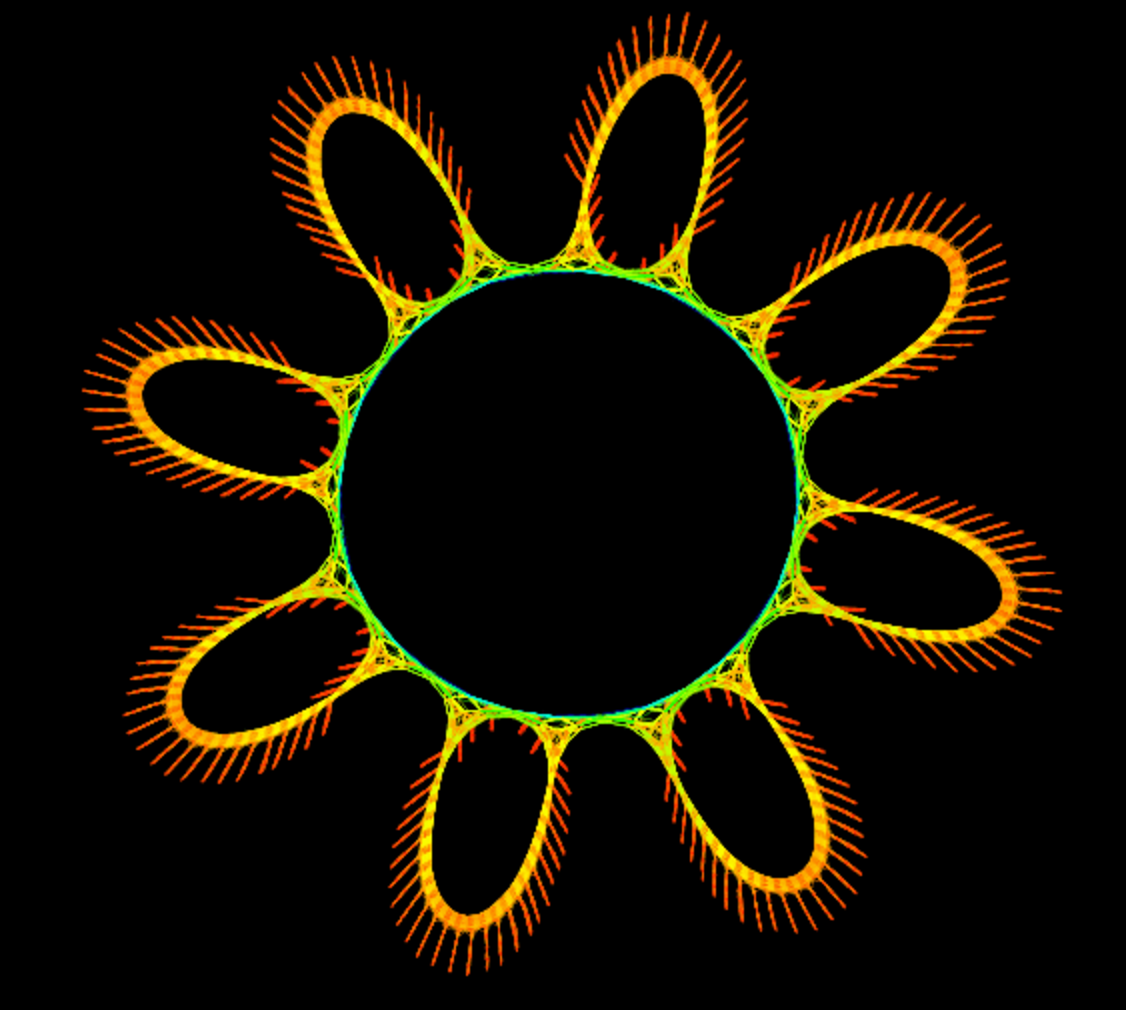
\includegraphics[scale = 0.7]{matrix1.png}}}
\centerline{Figure 1. Sparse Undirected Graph to be Partitioned}

\vspace{2mm}

\centerline {\frame{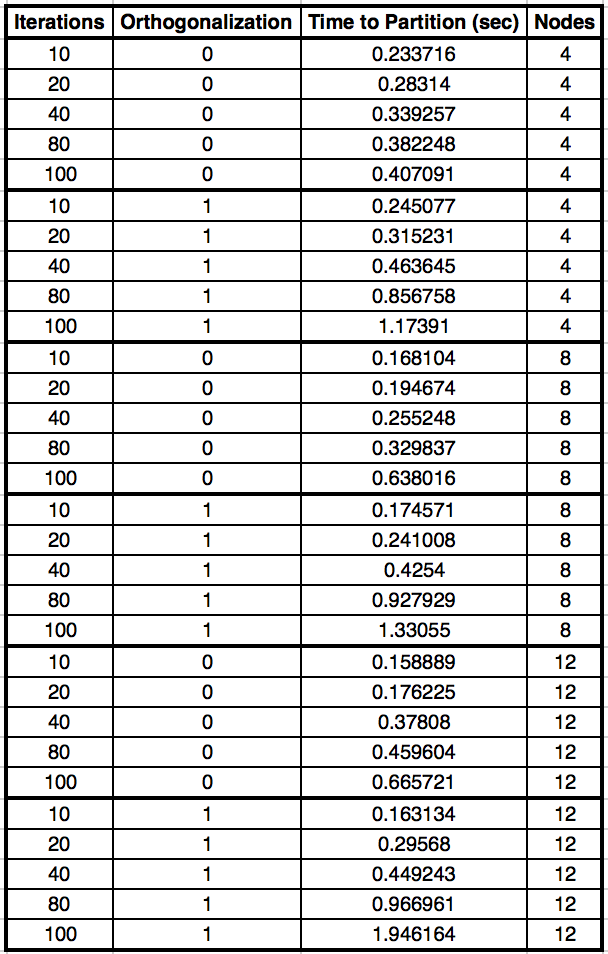
\includegraphics[scale = 1.0]{timingTable.png}}}
\centerline{Table 1. Timing Testing Results}

\vspace{2mm}

\centerline {\frame{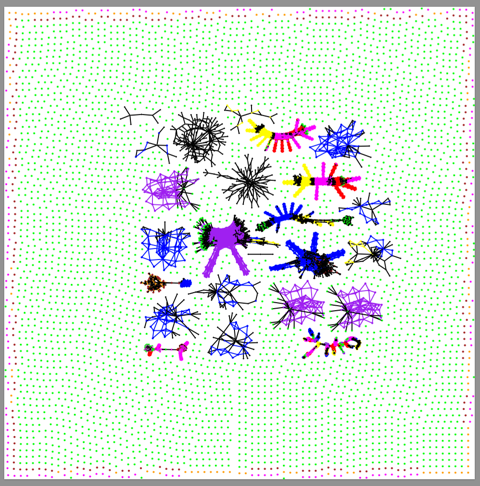
\includegraphics[scale = 1.2]{bigMatrixViz.png}}}
\centerline{Figure 2. Unexpected Visualization Results}

\vspace{2mm}

\centerline {\frame{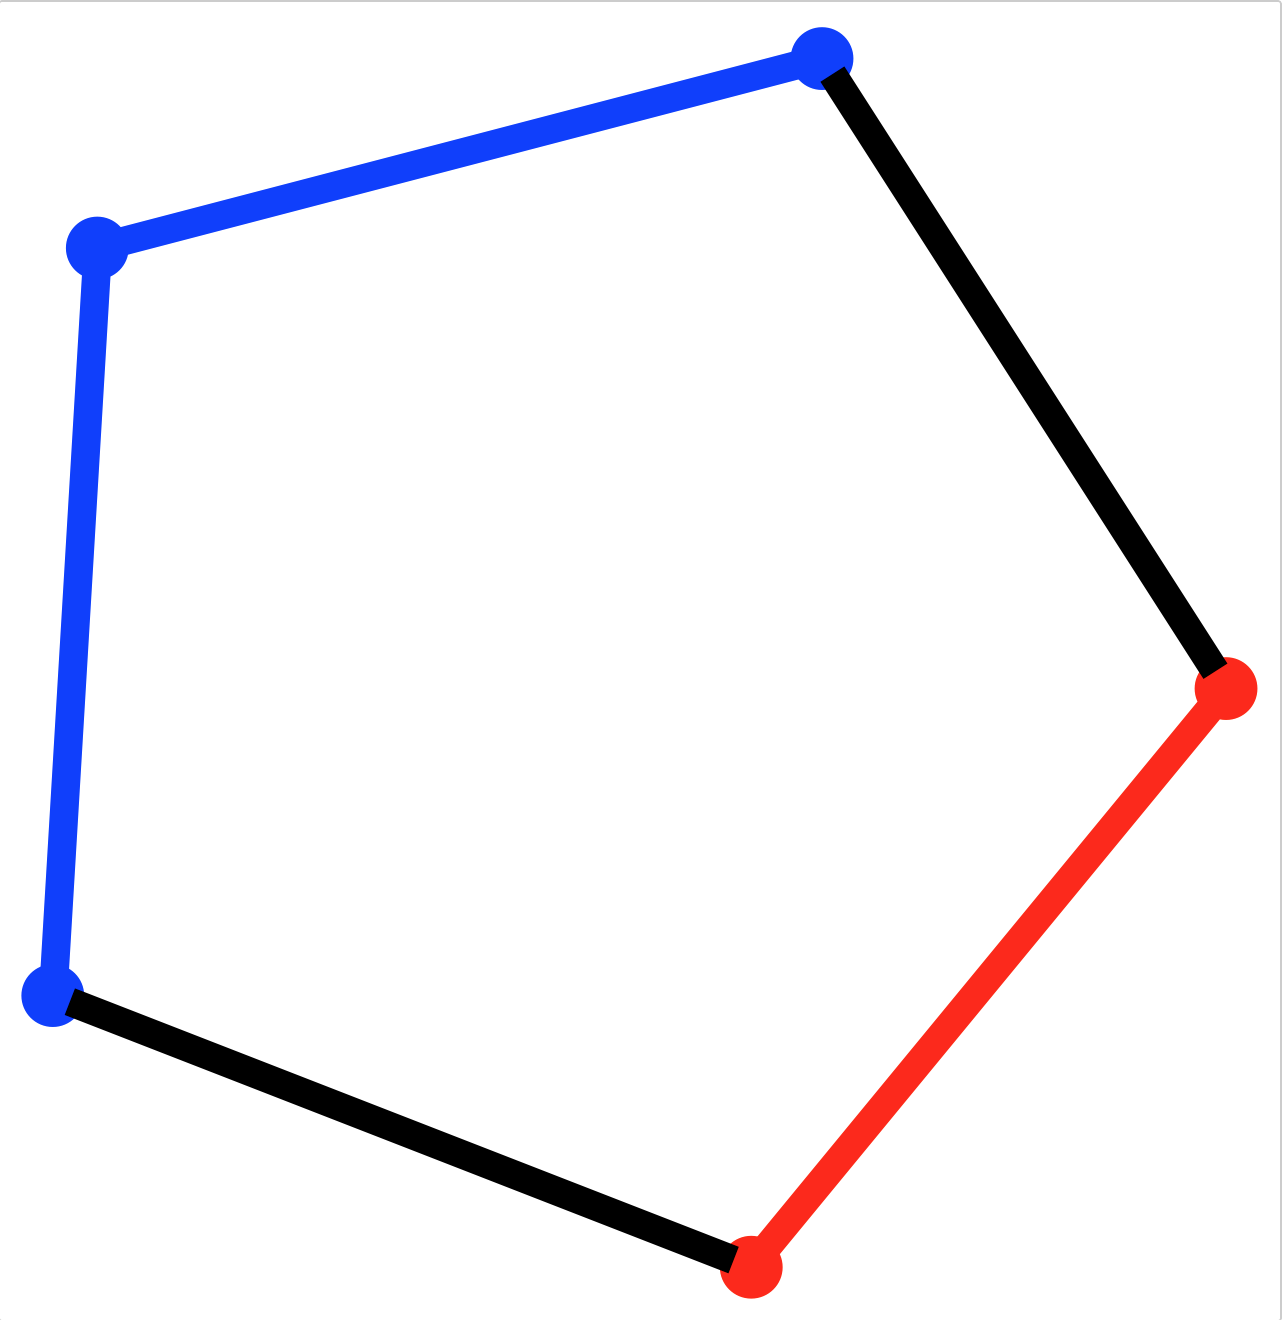
\includegraphics[scale = 0.5]{twoP.png}}}
\centerline{Figure 3. Pentagon Partition with 2 Processors}

\vspace{2mm}

\centerline {\frame{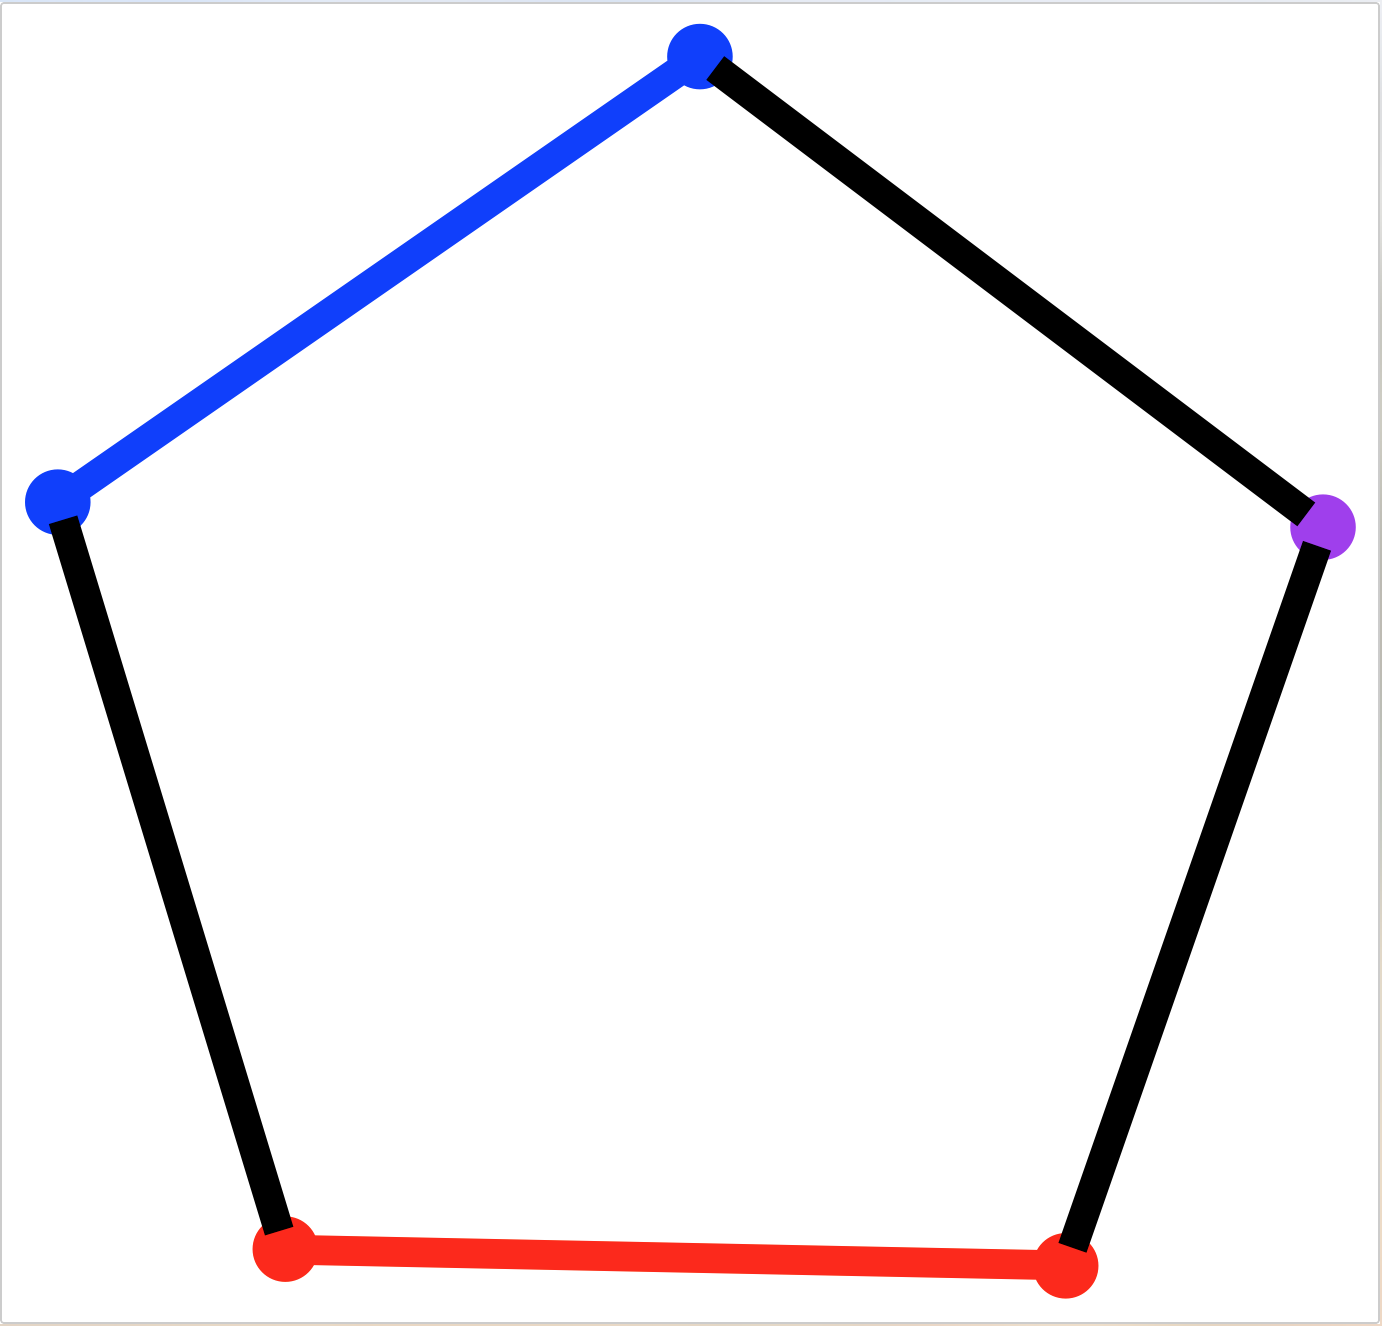
\includegraphics[scale = 0.5]{threeP.png}}}
\centerline{Figure 4. Pentagon Partition with 3 Processors}

\vspace{2mm}

\centerline {\frame{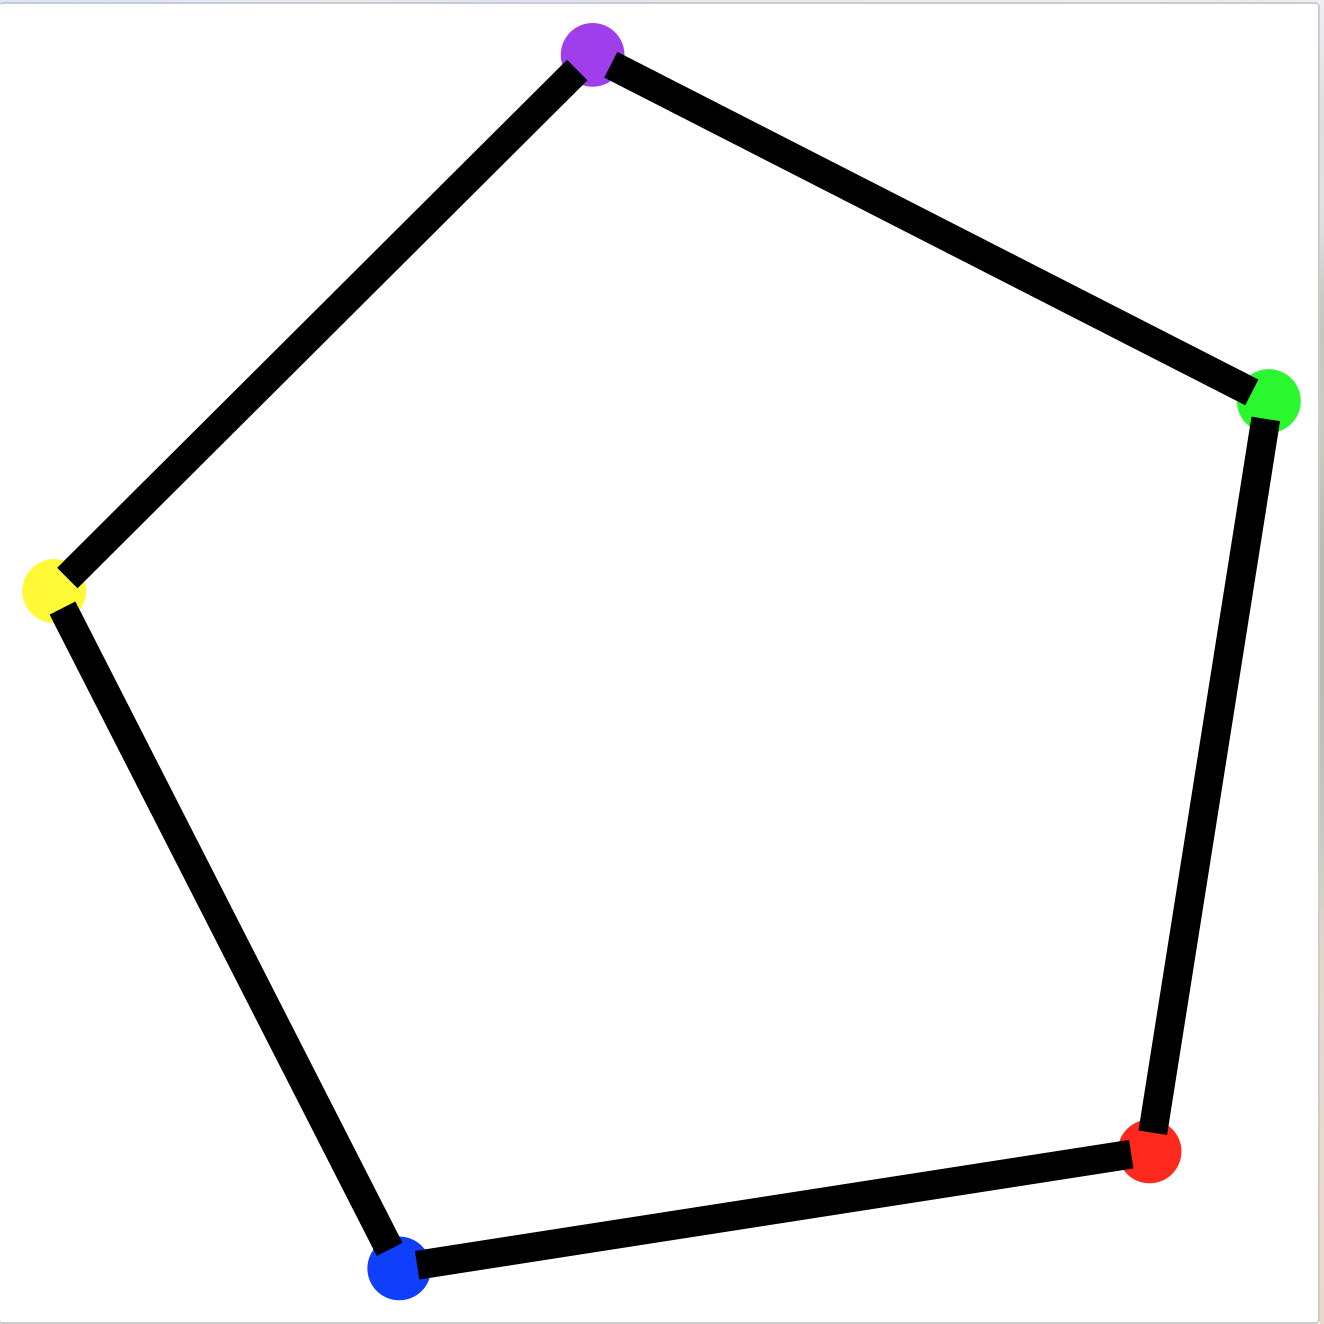
\includegraphics[scale = 0.5]{twelveP.png}}}
\centerline{Figure 5. Pentagon Partition with 12 Processors}

\section{Conclusions}

From the simple pentagon undirected graph, we can see the partition algorithm is working properly and yielding expected visualization results such as seeing two black lines when there were two processors. There should be two colored partitions, and two black lines as these represent the separations. We get the same expected results for three and twelve processors. However, when we tried to use this algorithm on a large undirected graph we obtained results that were not expected. We believe that this has to do with writing in to the same file from several processors at a time. We have been unsuccessful in finding this bug at this time.

Although the visualization results were unexpected for a large graph, we believe that the timing still represents the inner workings of the algorithm. These timings were done for 10, 20, 40, 80, and 100 Lanczos iterations with full orthogonalization (represented with a 1) and no orthogonalization (represented with a 0). On each processor with or without orthogonalization, the timing increases as iterations increases. This is an expected result as the algorithm is simply running for more time due to having more work to perform. Within each processor, the timing was also increased when full orthogonalization was performed. This is also an expected result due to, again, more work being done. Although the timing difference may not seem substantial because the algorithm is quite fast, but the relative differences can be almost double the time for full reorthogonalization. Unfortunately, we cannot see the visual results to determine if this added time would be worth the results. Across processors, adding more processors is helpful for time when the iterations are low, but when the iterations are up to 100 the timing starts to rise again due to communication costs. Again, it is unfortunate that we cannot see if this added time cost for more iterations would be worth the added time.

In conclusion, we have written a parallel Lanzcos graph partitioning algorithm that we have proved works for small graphs. We would need to revise how the files are written for the visualization software of choice or find another that has a better fit to the projects' needs. Although we cannot see the visual results of a large graph, the timing results do yield expected results which indicates the algorithm is working as expected.

\section{References}

\begin{enumerate}

\item The University of Florida Sparse Matrix Collection, T. A. Davis and Y. Hu, ACM Transactions on Mathematical Software, Vol 38, Issue 1, 2011, pp 1:1 - 1:25.

http://www.cise.ufl.edu/research/sparse/matrices.

\item James Demmel, Applied Numerical Linear Algebra, 1996

\item Emden R. Gansner and Stephen C. North, "An open graph visualization system and its applications to software engineering", SOFTWARE - PRACTICE AND EXPERIENCE, 2000, 30, 11, 1203--1233, Download from www.graphviz.org

\end{enumerate}

\end{document}
